\documentclass{article}

\def\npart {II}
\def\nyear {2017}
\def\nterm {Michaelmas}
\def\nlecturer{Dr H.\ Wilton}
\def\ncourse{Algebraic Topology}
\def\draft{Incomplete}
\ifx \nauthor\undefined
  \def\nauthor{Bhavik Mehta}
\else
\fi

\author{Based on lectures by \nlecturer \\\small Notes taken by \nauthor}
\date{\nterm\ \nyear}
\title{Part \npart\ -- \ncourse}

\usepackage[utf8]{inputenc}
\usepackage{amsmath}
\usepackage{amsthm}
\usepackage{amssymb}
\usepackage{enumerate}
\usepackage{mathtools}
\usepackage{graphicx}
\usepackage[dvipsnames]{xcolor}
\usepackage{tikz}
\usepackage{wrapfig}
\usepackage{centernot}
\usepackage{float}
\usepackage{braket}
\usepackage[hypcap=true]{caption}
\usepackage{enumitem}
\usepackage[colorlinks=true, linkcolor=mblue]{hyperref}
\usepackage[nameinlink,noabbrev]{cleveref}
\usepackage{nameref}
\usepackage[margin=1.5in]{geometry}

% Theorems
\theoremstyle{definition}
\newtheorem*{aim}{Aim}
\newtheorem*{axiom}{Axiom}
\newtheorem*{claim}{Claim}
\newtheorem*{cor}{Corollary}
\newtheorem*{conjecture}{Conjecture}
\newtheorem*{defi}{Definition}
\newtheorem*{eg}{Example}
\newtheorem*{ex}{Exercise}
\newtheorem*{fact}{Fact}
\newtheorem*{law}{Law}
\newtheorem*{lemma}{Lemma}
\newtheorem*{notation}{Notation}
\newtheorem*{prop}{Proposition}
\newtheorem*{question}{Question}
\newtheorem*{rrule}{Rule}
\newtheorem*{thm}{Theorem}
\newtheorem*{assumption}{Assumption}

\newtheorem*{remark}{Remark}
\newtheorem*{warning}{Warning}
\newtheorem*{exercise}{Exercise}

% \newcommand{\nthmautorefname}{Theorem}

\newtheorem{nthm}{Theorem}[section]
\newtheorem{nlemma}[nthm]{Lemma}
\newtheorem{nprop}[nthm]{Proposition}
\newtheorem{ncor}[nthm]{Corollary}
\newtheorem{ndef}[nthm]{Definition}

% Special sets
\newcommand{\C}{\mathbb{C}}
\newcommand{\N}{\mathbb{N}}
\newcommand{\Q}{\mathbb{Q}}
\newcommand{\R}{\mathbb{R}}
\newcommand{\Z}{\mathbb{Z}}

\newcommand{\abs}[1]{\left\lvert #1\right\rvert}
\newcommand{\norm}[1]{\left\lVert #1\right\rVert}
\renewcommand{\vec}[1]{\boldsymbol{\mathbf{#1}}}

\let\Im\relax
\let\Re\relax

\DeclareMathOperator{\Im}{Im}
\DeclareMathOperator{\Re}{Re}
\DeclareMathOperator{\id}{id}

\definecolor{mblue}{rgb}{0., 0.05, 0.6}



% preamble
\usetikzlibrary{knots,cd,decorations.pathmorphing}
\numberwithin{nthm}{subsection}
% and here we go!

% hjrw2
% orw notes
% hatchers book
\begin{document}
\maketitle

\tableofcontents

\section{Introduction}
Consider the trefoil and the trivial knot, called the unknot. We might be interested in asking whether or not these are the same, that is, can we untie a trefoil `knot' into a simple loop.

\begin{center}
    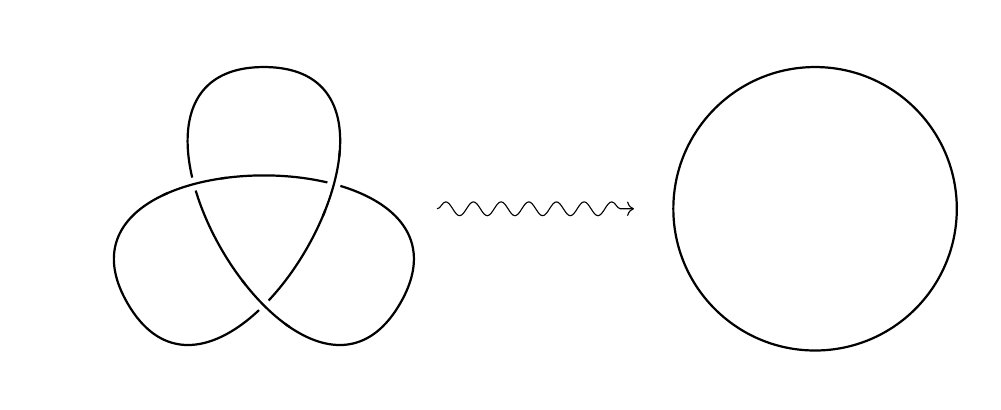
\begin{tikzpicture}
        \clip(-3,-2) rectangle (9, 2.5);
        \begin{knot}[
          clip width=6,
          consider self intersections=true, flip crossing=2,
          ]
          \strand[thick] (0,2)   .. controls +(2.5,0)   and +(120:-2.5) ..
                               (210:2) .. controls +(120:2.5) and +(60:2.5)  ..
                               (-30:2) .. controls +(60:-2.5) and +(-2.5,0)  ..
                               (0,2);
        \end{knot}

        \draw[->, decorate, decoration={snake, post length=4pt}] (2.2, 0.2) -- (4.7, 0.2);

        \draw[thick] (7, 0.2) circle [radius=1.8];
    \end{tikzpicture}
\end{center}
\paragraph{Question 1} Is the trefoil really a knot?

How do we make this precise?
We can think of the trefoil and the unknot as continuous embeddings from the circle $S^1$ into $\R^3$:
\begin{equation*}
    \begin{tikzcd}
        S^1 \arrow[r, hook, "f_i"] & \R^3
    \end{tikzcd}
\end{equation*}
where $f_0$ corresponds to the trefoil, and $f_1$ corresponds to the unknot.

\begin{center}
    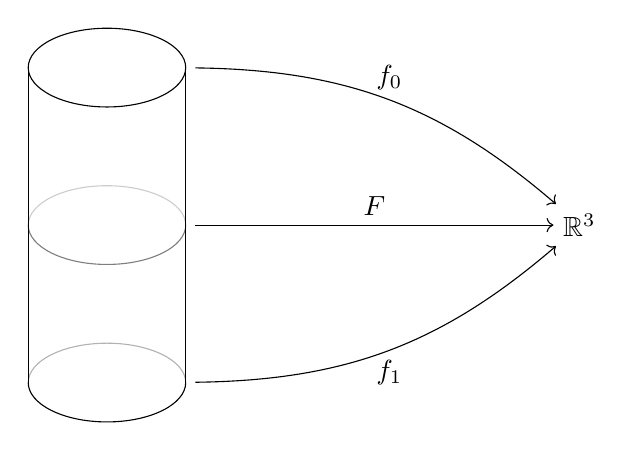
\begin{tikzpicture}[scale=0.5]
        \node (trefoil) at (2, 4) {};
        \node (unknot) at (2, -4) {};
        \node (middle) at (2, 0) {};
        \node (target) at (12, 0) {$\R^3$};

        \draw (0, 4) circle [x radius=2cm, y radius=1cm];
        \draw (unknot) arc [x radius=2cm, y radius=1cm, start angle=0, end angle=-180];
        \draw[opacity=0.3] (unknot) arc [x radius=2cm, y radius=1cm, start angle=0, end angle=180];

        \draw[opacity=0.2] (2, 0) arc [x radius=2cm, y radius=1cm, start angle=0, end angle=180];
        \draw[opacity=0.5] (2, 0) arc [x radius=2cm, y radius=1cm, start angle=0, end angle=-180];

        \draw (2, 4) -- (2, -4);
        \draw (-2, 4) -- (-2, -4);


        \draw[->] (trefoil) to[bend left=20] node[midway,above] {$f_0$} (target);
        \draw[->] (middle) -- (target) node[midway,above] {$F$};
        \draw[->] (unknot) to[bend right=20] node[midway,below] {$f_1$} (target);
    \end{tikzpicture}
\end{center}

\paragraph{Question 1 (precise)} Is there a continuous map
    \begin{equation*}
        F:S^1 \times [0, 1] \to \R^3
    \end{equation*}
    such that
    \begin{enumerate}[label=(\roman*)]
        \item $F(\theta, 0) = f_0(\theta)$, $F(\theta, 1) = f_1(\theta)$ $\forall \theta \in S^1$
        \item $F(\cdot, t_0): S^1 \to \R^3$ is injective, $\forall t_0 \in [0, 1]$
    \end{enumerate}

    We phrased unknotting as an \emph{extension problem}.  We can think about other, easier to state extension problems.

\paragraph{Question 2}
    Consider $S^2 = \set{\vec{x} \in \R^3 | \norm{x} = 1}$, and $D^3 = \Set{\vec{x} \in \R^3 | \norm{x} \leq 1}$ along with the natural inclusion $i$:
    \begin{equation*}
        \begin{tikzcd}
            S^2 \arrow[r, hook, "i"] & D^3
        \end{tikzcd}
    \end{equation*}
    Does there exist a continuous $f: D^3 \to S^2$ such that $f \circ i = \id_{S^2}$?
    \begin{equation*}
        \begin{tikzcd}
            S^2 \arrow[rr, "\id_{S^2}"] \arrow[rd, hook, "i"'] & & S^2 \\
                                                               & D^3 \arrow[ru, dashed, "?\exists f"']
        \end{tikzcd}
    \end{equation*}
    Intuitively, this question is asking us to find a map from the ball to the sphere that preserves every point on the sphere.
    Alternatively we can view this as extending the identity map on the sphere to a map from the ball.

    This seems like a hard question!  So, let's instead consider this analogous question in algebra.
    We take $S^2$ analogous to $\Z$, and $D^3$ analogous to $\{0\}$, the trivial group. From here, we get another question:

\paragraph{Question 3} Does there exist a group homomorphism $f: \{0\} \to \Z$ such that $\id_\Z = f \circ 0$?

    \begin{equation*}
        \begin{tikzcd}
            \Z \arrow[rr, "\id_{\Z}"] \arrow[rd, hook, "i"'] & & \Z \\
                                                             & \{0\} \arrow[ru, dashed, "?\exists f"']
        \end{tikzcd}
    \end{equation*}

    This question seems much easier to solve! This is the essence of algebraic topology - we turn difficult questions in topology into easy questions about algebra.

\subsection{Examples and conventions}

\begin{eg}
    \leavevmode
    \begin{itemize}
        \item Point $*$
        \item Circle $S^1$
        \item The circle generalises to the $n$-sphere, $S^{n-1} = \Set{x \in \R^n | \norm{x} = 1}$
            % TODO more damn pictures
        \item Which itself generalises into the genus-$g$ surface, $\Sigma_g$
        \item The torus can alternatively be found by identifying edges of a square, but by identifying them differently we can make a Klein bottle $K$
        \item Or the real projective plane $\mathbb{RP}^2$
    \end{itemize}

    % \begin{center}
    %     \begin{tikzpicture}
    %         \draw (0,0) circle [radius=2];

    %         \tikzset{shift={(5,0)}}
    %         \draw (0,0) circle [radius=2];
    %         \draw (2,0) arc [x radius=2, y radius=0.7, start angle=0, end angle=-180];
    %         \draw[opacity=0.3, very thin] (2,0) arc [x radius=2, y radius=0.7, start angle=0, end angle=180];

    %         \tikzset{shift={(0,-5)}}
    %         \draw (-1,0) to[bend left] (1,0);
    %         \draw (-1.2,.1) to[bend right] (1.2,.1);
    %         \draw[rotate=0] (0,0) ellipse (100pt and 50pt);
    %     \end{tikzpicture}
    % \end{center}
\end{eg}

In this course, the term map always refers to a continuous map.
To check that a map is continuous, we'll almost always use

\begin{lemma}[The Gluing Lemma\hypertarget{lem:gluingLemma}]
    If $X = C_1 \cup C_2$ with $C_i$ closed, and $f: X \to Y$ is a function such that $f|_{C_1}$ and $f|_{C_2}$ are both continuous, then $f$ is continuous.
\end{lemma}

\begin{proof}
    Let $D \subseteq Y$ be closed.  Then
    \begin{equation*}
        f^{-1}(D) = (f|_{C_1})^{-1} (D) \cup (f|_{C_2})^{-1} (D)
    \end{equation*}
    is a finite union of closed sets, hence is closed.  Therefore, $f$ is continuous.
\end{proof}

\subsection{Cell complexes}
There are the spaces we can build by gluing.  The \emph{basic operation} we use is to attach an $n$-dimensional disc, as shown in the non-existent diagram. % TODO: gluing diagram
Formally, if $f: S^{n-1} \to X$ is a continuous map, then we produce
\begin{equation*}
    (X \sqcup D^n) / \sim
\end{equation*}
where $\sim$ is an equivalence relation: $Y \sim f(y)$, for $y \in S^{n-1}$ and $f(y) \in X$.
\begin{defi}[Cell complexes]
    We define cell complexes by induction:
    \begin{enumerate}[label=(\roman*)]
        \item A zero-dimensional cell complex is a finite discrete topological space
        \item An $n$-dimensional cell complex is constructed from an $(n-1)$ dimensional cell complex $X$ by attaching finitely many $n$-dimensional discs to $X$.
    \end{enumerate}
\end{defi}

\clearpage

\section{Homotopy and the Fundamental Group}
\paragraph{Main question} How can we prove that $X \ncong Y$?
The basic idea is to associate algebraic objects (for instance groups) to $X, Y$.

\subsection{Homotopy}
Throughout, we will denote $I = [0, 1] \subseteq \R$.

% def 2.1.1
\begin{ndef}\hypertarget{def:homotopy}
    Let $f, g: X \to Y$ be maps. A \textbf{homotopy} from $f$ to $g$ is a continuous map $H: X \times I \to Y$ such that $H(x, 0) = f(x)$ and $H(x, 1) = g(x) \; \forall x \in X$.
    We say that $f$ and $g$ are \textbf{homotopic}, and write $f \simeq g$ (or $f \simeq_H g$).
\end{ndef}

\begin{ndef}\hypertarget{def:homotopyRel}
    If $A \subseteq X$ and $\forall a \in A, \forall t \in I$, $H(a, t) = f(a) = g(a)$, then we say \textbf{$f$ is homotopic to $g$ relative to $A$} and we write $f \simeq g$ rel $A$.
\end{ndef}

% prop 2.1.2
\begin{nprop}
    The relation $\simeq$  (rel $A$) is an equivalence relation.
\end{nprop}

\begin{proof}
    Reflexivity and symmetry are easy exercises, so they are omitted.  Transitivity: we have $f, g, h: X \to Y$, where $f \simeq_H g$ and $g \simeq_H' h$, and our goal is to build a homotopy $f \simeq h$.

    colourful pictures go here

    From the diagram, it's clear that the required homotopy is given by
    \begin{align*}
        H'' : X \times I &\to Y \\
        (x, t) &\mapsto
        \begin{cases}
            H(x, 2t) & 0 \leq t \leq \frac12 \\
            H'(x, 2t-1) & \frac12 \leq t \leq 1
        \end{cases}
    \end{align*}
    This is continuous from the gluing lemma.
\end{proof}

\begin{ndef}\hypertarget{def:homotopyEq}
    If we have $f: X \to Y$ and $g: Y \to X$ (diagram) with $g \circ f \simeq \id_X$ and $f \circ g \simeq \id_Y$, then we say that $X$ and $Y$ are \textbf{homotopy equivalent}, and $f, g$ are \textbf{homotopy equivalences}, and we write $X \simeq Y$.
\end{ndef}

\begin{eg}
    Take $X = \R^n$ and $Y = *$. Consider the trivial map $r: \R^n \to *$ and $i: * \to \R^n$, $i(*) = 0$. Then $r \circ i = \id_*$ and $i \circ r = 0: \R^n \to \R^n$
    Let $H: R^n \times I \to \R^n$ $(x, t) \mapsto tx$, so for $t=0$, H(., 0) = 0 and for $t=1$, $H(., 1) = \id_{\R^n}$.
\end{eg}

\begin{eg}
    This time, consider the spaces $\R^2 \setminus {0}$ and $S^1$, and the maps $r(x) = \frac{x}{\norm{x}}$  and inclusion $i$.  Then $r \circ i = \id_{S^1}$ and we can use the homotopy $H(x, t) = tx + (1-t) \frac{x}{\norm{x}}$ to show $i \circ r \simeq \id_{\R^2 \setminus {0}}$.  So, $\R^2 \setminus \{0\}$ and $S^1$ are homotopy equivalent.
\end{eg}

\begin{ndef}
    If $X$ is homotopy equivalent to a point, we say that $X$ is \textbf{contractible}.
\end{ndef}

% def 2.1.7
\begin{nlemma}
    If
    [diagram]
    are maps with $f_0 \simeq_H f_1$ and $g_0 \simeq_H'$ then $g_0 \circ f_0 \simeq g_1 \circ f_1$.
\end{nlemma}

\begin{proof}
    We show that both are homotopic to $g_0 \circ f_1$.  $g_0 \circ f_0 \simeq g_0 \circ f_1$ via $g_0 \circ H$ and $g_0 \circ f_1 \simeq g_1 \circ f_1$ via $H'(f_1(\cdot), \cdot)$.
\end{proof}

% prop 2.1.8
\begin{prop}
    Homotopy equivalence is an equivalence relation of spaces.
\end{prop}

\begin{proof}
    Symmetry and reflexivity are trivial. Transitivity [diagram]
    Suppose these are homotopy equivalences. We need to show $g \circ g' \circ f' \circ f \simeq \id_X$ and $f' \circ f \circ g \circ g' \simeq \id_Z$.
    Now,
    \begin{equation*}
        g \circ (g' \circ f') \circ f \simeq g \circ \id_Y \circ f \simeq g \circ f \simeq \id_X \\
    \end{equation*}
    and
    \begin{equation*}
        f' \circ (f \circ g) \circ g' \simeq f' \circ \id_Y \circ g' \simeq f' \circ g' \simeq \id_Z \\
    \end{equation*}
\end{proof}

% defi 2.1.9
\begin{ndef}[\hypertarget{def:defRet}{Deformation retraction}]
    If $i: A \hookrightarrow X$ is an inclusion, $r: X \to A$ is a continuous map such that $r \circ i = \id_A$ and $i \circ r \simeq \id_X$ rel $A$ then $A$ is called a \textbf{deformation retract} of $X$, and $r$ is a \textbf{deformation retraction}.
\end{ndef}

\begin{ndef}
    If $r: X \to A$ is a map such that $ r \circ i = \id_A$, then $A$ is a \textbf{retract} and $r$ is a retraction.
\end{ndef}

\begin{eg}
    If $X \neq \emptyset$, then for any $x \in X$, $r: X \to \{x\}$ is a retraction.
\end{eg}

Recall our basic goal was to prove that $X \not\simeq Y$ or that $X \not \cong Y$, and we will develop tools to do this.  For instance we can think about the spaces $X = *$ and $Y = * \sqcup *$.

% 2.2
\subsection{Paths}

% 2.2.1
\begin{ndef}
    A \textbf{path} in a space $X$ is a map $\gamma: I \to X$.
    A \textbf{path from $x_0$ to $x_1$} is such a map with $\gamma(0) = x_0$ and $\gamma(1) = x_1$, which we can denote by $\gamma: x_0 \leadsto x_1$.
    If $x_0 = x_1$, we say that $\gamma$ is a \textbf{loop}.
\end{ndef}

If $\gamma_0: x_0 \leadsto x_1$ and $\gamma_1: x_1 \leadsto x_2$ then the contraction of $\gamma_0$ and $\gamma_1$ is
\begin{equation*}
    (\gamma_0 \cdot \gamma_1) (t) =
    \begin{cases}
        \gamma_0(2t) & 0 \leq t \leq \frac12 \\
        \gamma_1(2t-1) & \frac12 \leq t \leq 1
    \end{cases}
\end{equation*}

If $\gamma: I \to X$ is a path, the inverse path $\gamma^{-1} = \bar{\gamma}$, given by $\bar{\gamma}(t) = \gamma(1-t)$.
For any $x_0 \in X$, the constant path
\begin{align*}
    C_{x_0}: I &\to X \\
             t &\mapsto x_0
\end{align*}

% defi 2.2.2
\begin{ndef}\hypertarget{def:pathComp}{Path components}
    If there is a path $\gamma:x_0 \leadsto x_1$, then we write $x_0 \sim x_1$.  By the above, this is an equivalence relation on $X$.  We write
    \begin{equation*}
        \pi_0(X) = X/\sim
    \end{equation*}
    and call the equivalence classes $[x]$ the \textbf{path components} of X.
    If there is only one path component, we say $X$ is path connected.
\end{ndef}

What's more, if $f: X \to Y$ is a map, we can define
\begin{align*}
    \pi_0(f): \pi_0(X) &\to \pi_0(Y)
    [x] &\mapsto [f(x)]
\end{align*}
It's easy to see that this is well-defined.

% prop 2.2.3
\begin{nprop}
    For [diagram] continuous maps.
    \begin{enumerate}[label=(\roman*)]
        \item if $f_0 \simeq f_1$, then $\pi_0(f_0) = \pi_0(f_1)$
        \item $\pi_0(f \circ f_0) = \pi_0(g) \circ \pi_0(f_0)$
        \item $\pi_0(\id_X) = \id_{\pi_0(X)}$
    \end{enumerate}
\end{nprop}

\begin{proof}
    \leavevmode
    \begin{enumerate}[label=(\roman*)]
        \item Let $f_0 \simeq_H f_1$. For any $x \in X$, $H(x, \cdot): I \to Y$ is a path from $f_0(x) to f_1(x)$, hence $[f_0(x)] = [f_1(x)]$, and therefore $\pi_0(f_0)([x]) = \pi_0(f_1)([x])$.
    \end{enumerate}
    (ii) and (iii) are immediate.
\end{proof}

\begin{eg}[Toy example]
    We try to show $* \not \simeq * \sqcup *$.  First, see that $1 = \abs{\pi_0(*)}$ and $\abs{\pi_0(* \sqcup *)} = 2$. Suppose we have a pair of homotopy equivalences between $X$ and $Y$ called $f, g$.
    Then $\pi_0(f) \circ \pi_0(g) = \pi_0(f \circ g) = \pi_0(\id_*) = \id_{\pi_0(*)}$. Likewise, $\pi_0(g) \circ \pi_0(f) = \id_{\pi_0(* \sqcup *)}$ hence $\pi_0(f)$ is a bijection, $\implies 1=2$.
\end{eg}

Our next goal is to fix up the group axioms for paths. We could allow unrestricted homotopies of paths, but then all paths would be homotopic. Instead we fix the endpoints.

% defi 2.2.7
Paths $\gamma, \gamma': I \to X$ are \textbf{homotopic as paths} if $\gamma \simeq \gamma'$ rel $\{0, 1\}$.

Homotopy of paths and concatenations interact nicely.

% lemma 2.2.8
\begin{nlemma}
    If $\gamma_0, \gamma_0': x_0 \leadsto x_1$, (vert) $\gamma_1, \gamma_1': x_1 \leadsto x_2$ and $\gamma_0 \simeq \gamma_0'$, $\gamma_1 \simeq \gamma_1'$ as paths then $\gamma_0 \cdot \gamma_1 \simeq \gamma_0' \cdot \gamma_1'$.
\end{nlemma}

\begin{proof}[Sketch]
    Suppose $\gamma_0 \simeq_{H_0} \gamma_0'$ and $\gamma_1 \simeq_{H_1} \gamma_1'$.
    The diagram shows the homotopy of paths we are looking for.
\end{proof}

% prop 2.2.9
\begin{nprop}
    Let $\gamma_0:x_0 \leadsto x_1$, $\gamma_1: x_1 \leadsto x_2$, $\gamma_2: x_2 \leadsto x_3$.
    Then
    \begin{enumerate}[label=(\roman*)]
        \item $(\gamma_0 \cdot \gamma_1) \cdot \gamma_2 \simeq \gamma_0 \cdot (\gamma_1 \cdot \gamma_2)$
        \item $\gamma_0 \cdot c_{x_1} \simeq \gamma_0 \simeq c_{x_0} \cdot \gamma_0$
        \item $\gamma_0 \cdot \overline{\gamma_0} \simeq c_{x_0}$, $\overline{\gamma_0} \cdot \gamma_0 \simeq c_{x_1}$
    \end{enumerate}
\end{nprop}

\begin{proof}
    \leavevmode
    \begin{enumerate}[label=(\roman*)]
        \item
                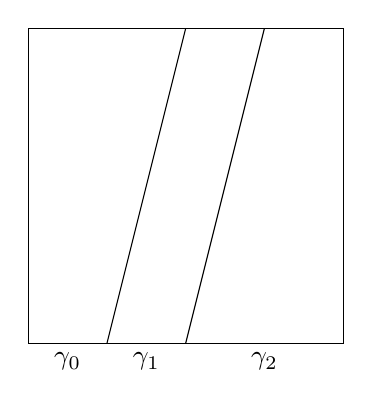
\begin{tikzpicture}[{baseline=(current bounding box.north)}]
                    \draw (0, 0) rectangle (4, 4);
                    \draw (1, 0) -- (2, 4);
                    \draw (2, 0) -- (3, 4);

                    % \node[below] at (1, 0) {$x_1$};
                    % \node[below] at (2, 0) {$x_2$};
                    % \node[above] at (2, 4) {$x_1$};

                    \node[below] at (0.5, 0) {$\gamma_0$};
                    \node[below] at (1.5, 0) {$\gamma_1$};
                    \node[below] at (3, 0) {$\gamma_2$};
                \end{tikzpicture}

        \item
        \item We prove the first only, since they are clearly equivalent.
    \end{enumerate}
\end{proof}

\subsection{The Fundamental Group}

\begin{nthm}
    For $X$ a space, $x_0 \in X$, if $\pi_1 (X, x_0)$ denotes the set of homotopy classes of loops starting and ending at $x_0$, then concatenation defines a group structure on $\pi_1(X, x_0)$.
\end{nthm}

\begin{proof}
    Lemma 2.2.8 gives us that multiplication is well defined, and proposition 2.2.9 shows that the group axioms hold.
\end{proof}

\begin{defi}
    A \textbf{based space} is a pair $(X, x_0)$, where $X$ is a space and $x_0 \in X$. A \textbf{map of based spaces} $f:(X, x_0) \to (Y, y_0)$ is a map $f:X \to Y$ such that $f(x_0) = y_0$. A \textbf{based homotopy} is a homotopy $H:X \times I \to Y$ rel $\{x_0\}$.
\end{defi}

\begin{defi}
    If $f(X, x_0) \to (Y, y_0)$ is a map of based spaces, we get a natural map
    \begin{align*}
        \pi_1(f) : \pi(X, x_0) &\to \pi(Y, y_0)
        [\gamma] &\mapsto [f \circ \gamma]
    \end{align*}
    and it's easy to see that this is well defined.
\end{defi}

\begin{nprop}
    Let $f: (X, x_0) \to (Y, y_0)$ be a map of based spaces.
    \begin{enumerate}[label=(\roman*)]
        \item $\pi_1(f)$ is a group homomorphism
        \item If $f \simeq f'$ rel $\{x_0\}$ then $\pi_1(f) = \pi_1(f')$.
        \item If $g: (Y, y_0) \to (Z, z_0)$ is a based map then $\pi_1(g \circ f) = \pi_1(g) \circ \pi_1(f)$
        \item $\pi_1(\id_{X, x_0}) = \id_{\pi(X, x_0)}$
    \end{enumerate}
\end{nprop}

\begin{proof}
    Easy exercise.
\end{proof}

\begin{cor}
    If $(X, x_0)$ and $(Y, y_0)$ are \emph{based} homotopy equivalent, then \begin{equation*}\pi_1(X, x_0) \cong \pi_1(Y, Y_0)\end{equation*}.
\end{cor}

Let's investigate the effect of our choice of basepoint.

If we have a space $X$ which is not path connected, then the groups $\pi_1(X, x_0)$ and $\pi_1(X, x_1)$ can be completely unrelated if $x_0$ and $x_1$ are in different path components.

$\pi_1(X, x_0) \to \pi_1(X, x_1)$
$[\gamma] \mapsto [\overline{u} \cdot \gamma \cdot u]$
This is well-defined by lemma 2.2.8

% 2.3.4
\begin{prop}
    Let $u: x_0 \leadsto x_1$ be a path in $X$.
    \begin{enumerate}[label=(\roman*)]
        \setcounter{enumi}{0}
        \item If $u \simeq u'$ as paths then $u_{\#} = u_{\#}'$
        \item $(c_{x_0})_{\#} = \id_{\pi_1(X, x_0)}$
        \item If $v: x_1 \leadsto x_2$, thus
            \begin{equation*}
                (u \cdot v)_{\#} = v_{\#} \circ u_{\#}
            \end{equation*}

        \item Suppose $f:X \to Y$ is a continuous map with $f(x_1) = y_1$
                Then the diagram commutes.
        \item If $u$ is a loop, then $u_{\#}: \pi_1(X, x_0) \to \pi_1(X, x_0)$ is the automorphism of $\pi_1(X, x_0)$ given by conjugation by $[u]$.
    \end{enumerate}
\end{prop}

\begin{proof}
    Immediate applications of lemma (2.2.8) and prop (2.2.9).
\end{proof}

\begin{cor}
    If $X$ is path connected then $\forall x_0, x_1 \in X$,
    \begin{equation*}
        \pi(X, x_0) \cong \pi(X, x_1)
    \end{equation*}
\end{cor}

\begin{warning}
    This isomorphism is not canonical. In general, different choices of path change our isomorphism by a conjugation.
\end{warning}

The goal is to show that the fundamental group is an invariant of \emph{homotopy equivalence}.
% TODO diagram

Let $f, g: X \to Y$ be maps, $x_0 \in X$ and suppose $f \not\simeq_{H} g$. Then, $u(t) = H(x_0, t)$ is a path in $Y$ from $f(x_0) \leadsto g(x_0)$.

\begin{equation*}
    \begin{tikzcd}
        & \pi_1(Y, f(x_0)) \arrow[dd, "u_{\#}"]\\
        \pi_1(X, x_0) \arrow[ur, "f_*"] \arrow[dr, "g_*"] & \\
                                                          & \pi_1(Y, g(x_0))
    \end{tikzcd}
\end{equation*}

% lemma 2.3.6
\begin{lemma}
    For $f, g, u$ as above, $g_* = u_{\#} \circ f_*$ (the diagram commutes).
\end{lemma}

\begin{proof}
    Let $\gamma$ be a loop in $X$ based at $x_0$. We need to prove that
    \begin{equation*}
        (g \circ \gamma) \simeq \overline{u} \cdot (f \circ \gamma) \cdot u
    \end{equation*}
    as paths.

    Consider
    \begin{align*}
        I &\times I & &\to & X &\times I & &\xrightarrow{H} & Y \\
        (s&, t) & &\mapsto & (\gamma(s)&, t)
    \end{align*}

    Together, this gives $F(s, t) = H(\gamma(s), t)$.
    % TODO: picture

    We can see that
    \begin{align*}
        F(s, 0) &= f \circ \gamma(s)\\
        F(s, 1) &= g \circ \gamma(s) \\
        F(0, t) &= H(\gamma(0), t) = H(x_0, t) = u(t) \\
        F(1, t) &= H(\gamma(1), t) = H(x_0, t) = u(t)
    \end{align*}

    Consider the two paths in the square $I \times I$ illustrated:
    \begin{align*}
        l_+ : I \to I \times I \\
        l_- : I \to I \times I
    \end{align*}
    and note that $g \circ \gamma = F \circ l_+$ while $\overline{u} \cdot (f \circ \gamma) \cdot u = F \circ l_-$.

    So, we can let
    \begin{align*}
        L: I \times I &\to I \times I \\
        (s, t) &\mapsto t l_+(s) + (1-t) l_-(s)
    \end{align*}

    This is a homotopy of paths $l_+ \simeq l_-$.

    Therefore, $F \circ L$ is a homotopy of paths from $g \circ \gamma$ to $\overline{u} \cdot (f \circ \gamma) \cdot u$ as required.
\end{proof}

% thm 2.3.7
\begin{thm}
    If
        \begin{tikzcd}
            X \arrow[r, bend left, "f"] & Y \arrow[l, bend left, "g"]
        \end{tikzcd}
    is a pair of homotopy equivalences, then for any $x_0 \in X$
    \begin{equation*}
        f_*: \pi(X, x_0) \to \pi(Y, f(x_1))
    \end{equation*}
    is an isomorphism.
\end{thm}

\begin{proof}
    Let $g \circ f \simeq_H \id_X$ and let $u(t) = H(x_0, t)$. By lemma (2.3.6),
    \begin{align*}
        g_* \circ f_* &= (g \circ f)_* \\
                      &= u_{\#} \circ (\id_X)_* \\
                      &= u_{\#}
    \end{align*}
    an isomorphism, so $f_*$ is injective.

    Likewise, using the other homotopy, we get that $f_* \circ g_*$ is an isomorphism and so $f_*$ is surjective.
\end{proof}

\begin{eg}
    Take $X = * = \{x_0\}$. Then $\pi_1(X, x_0) \cong 1$, the trivial group.  By the Theorem, this holds for \textbf{any} contractible space X.
\end{eg}

\begin{defi}[Simply connected\hypertarget{def:simplyConnected}]
    If $X$ is path-connected and $\pi_1(X, x_0) \cong 1$ then we say that $X$ is \textbf{simply connected}.
\end{defi}

We have many examples of spaces with trivial fundamental group, but can we find a space $X$ such that $\pi_1 X \ncong 1$?

\clearpage
\section{Covering Spaces}

\subsection{Covering spaces}

% defi 3.1.1
\begin{ndef}
    A \textbf{covering map} $P: \widetilde{X} \to X$ is a map such that any point $x \in X$ has a neighbourhood $U$ such that
    \begin{equation*}
        p^{-1}(U) = \bigsqcup_{\alpha \in \Lambda} V_\alpha
    \end{equation*}
    such that $p|_{V_\alpha}: V_\alpha \to U$ are homeomorphisms. Our covering maps will always be surjective.

    We will often just say $\widetilde{X}$ is a \textbf{covering space}.

    We say that $U$ is \textbf{evenly covered}.
\end{ndef}

\begin{eg}
    \leavevmode
    \begin{itemize}
        \item Homeomorphisms
        \item Products of covering maps are covering maps
        \item Take $X = S^1 \subseteq \C$, and $\widetilde{X} = \R$. Then consider
            \begin{align*}
                p: \R &\to S^1 \\ t &\mapsto \exp(2 \pi i t)
            \end{align*}

            For any $x \in S^1$, on a small neighbourhood of $x$, for any $\widetilde{x} \in p^{-1}(x)$, we can write down an inverse of $p$ using $\sin^{-1}, \cos^{-1}$.
        \item Take $\widetilde{X} = S^1,\, X = S^1$ as subsets of $\C$. Consider
            \begin{align*}
                p_n: S^1 &\to S^1 \\
                z &\mapsto z^n
            \end{align*}
        \item Let $\widetilde{X} = S^2$, and let $x \sim y \iff x = \pm y$. Then, use $X = \widetilde{X}/\sim$, the real projective plane, $\R P^2$ be the quotient map, which is a covering map.

            \begin{center}
                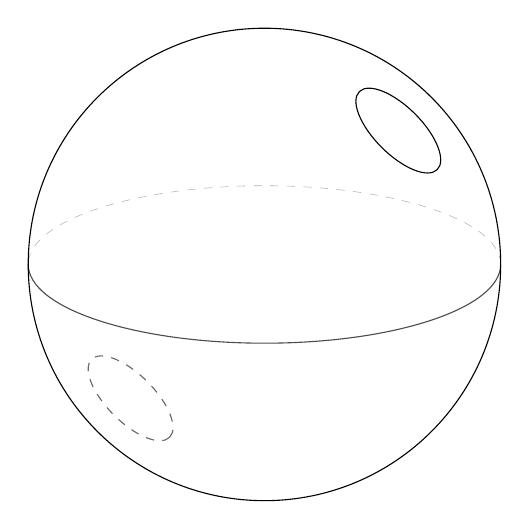
\begin{tikzpicture}
                    \draw (0, 0) circle[radius=3];
                    \draw[opacity=0.7] (3,0) arc [x radius=3, y radius=1, start angle=0, end angle=-180];
                    \draw[dashed, opacity=0.3, very thin] (3,0) arc [x radius=3, y radius=1, start angle=0, end angle=180];
                    \draw (1.7, 1.7) ellipse [rotate=-45, x radius=0.7, y radius=0.3];
                    \draw[dashed, opacity=0.6] (-1.7, -1.7) ellipse [rotate=-45, x radius=0.7, y radius=0.3];
                \end{tikzpicture}
            \end{center}
    \end{itemize}
\end{eg}

% def 3.1.7
\begin{defi}
    If $f: Y \to X$ is a map and $p: \widetilde{X} \to X$ is a covering map. The \textbf{lift} of $f$ along $p$ is a map $\widetilde{f}: Y \to \widetilde{X}$ such that $p \circ \widetilde{f} = f$.
\end{defi}

% lem 3.1.8
\begin{lemma}[Uniqueness for lifts]
    Let $f: Y \to X$ be a map, $\widetilde{X} \to X$ a covering map. SUppose $\widetilde{f_0}, \widetilde{f_1}$ are both lifts of $f$. Then
    \begin{equation*}
        S = \set{y \in Y \mid \widetilde{f_0}(y) = \widetilde{f_1}(y)}
    \end{equation*}
    is both open and closed. So, if $Y$ is connected, $\widetilde{f_0}$ and $\widetilde{f_1}$ agree everywhere or nowhere. In particular, any lift $\widetilde{f}$ is determined by its value at \emph{one} point of $Y$.
\end{lemma}

\begin{proof}
    First show $S$ is open. Let $y \in S$, so $\widetilde{f_0}(y) = \widetilde{f_1}(y)$.
    We need to find a neighbourhood of $y$ contained in $S$.
    Let $U$ be an evenly covered neighbourhood of $f(y)$.
    Then $\phi^{-1}(U) = \bigsqcup_{\beta \in \Lambda} V_\beta$.
    Let $\beta_0$ be such that $\widetilde{f_0}(y) = \widetilde{f_1}(y) \in V_{\beta_0}$.

    Consider $\widetilde{f_0}^{-1}(V_{\beta_0}), \widetilde{f_1}^{-1}(V_{\beta_0})$ neighbourhoods of $y$.
    Let $N = \widetilde{f_0}^{-1}(V_{\beta_0}) \cap \widetilde{f_1}^{-1}(V_{\beta_0})$.
    Now, $\widetilde{f_0}^{-1}(N), \widetilde{f_1}^{-1}(N) \subseteq V_{\beta_0}$, so
    \begin{equation*}
        p |_{V_{\beta_0}} \circ \widetilde{f_0}(N), p |_{V_{\beta_0}} \circ \widetilde{f_1}(N) \subseteq U
    \end{equation*}

    Therefore, $\widetilde{f_0}|_N = (p |_{V_{\beta_0}})^{-1} \circ f = \widetilde{f_1}|_N$, so $N \subseteq S$.


    Next we must show $S$ is closed.  Let $y \notin S$, so $\widetilde{f_0}(y) \neq \widetilde{f_1}(y)$.
    Let $U$ be an evenly covered neighbourhood of $f(y)$.
    Then $\phi^{-1}(U) = \bigsqcup_{\beta \in \Lambda} V_\beta$.

    Since $\widetilde{f_0}(y) \neq \widetilde{f_1}(y)$, $\exists \beta \neq \gamma$ such that $\widetilde{f_0}(y) \in V_{\beta}, \, \widetilde{f_1}(y) \in V_{\gamma}$.

    Again, let $N = \widetilde{f_0}^{-1}(V_{\beta}) \cap \widetilde{f_1}^{-1}(V_{\gamma})$.
    Since $\widetilde{f_0}(N) \subseteq V_\beta$ is disjoint from $\widetilde{f_1}(N) \subseteq V_\gamma$ we see that $N \subseteq S^c$.
\end{proof}

Having proved uniqueness, we next turn to existence in the case $Y = I$, the case of paths.

% lem 3.1.10
\begin{lemma}[Path lifting lemma]
    Let $P: \widetilde{X} \to X$ be a covering map with $\gamma:I \to X$ a path, and $\widetilde{x_0} \in \widetilde{X}$ such that $p(\widetilde{x_0}) = x_0 = \gamma(0)$.
    Then there is a unique lift $\widetilde{\gamma}$ such that $\widetilde{\gamma}(0) = \widetilde{x_0}$.
\end{lemma}

% missing stuff!

% lemma 3.1.15
\begin{lemma}
    Let $p:(\widetilde{X}, \widetilde{x_0}) \to (X, x_0)$ be a (based) covering map with $X$ path-connected. Then:
    \begin{enumerate}[label=(\roman*)]
        \item $\widetilde{X}$ is path-connected iff $\pi_1(X, x_0)$ acts transitively on $p^{-1}(x_0)$;
        \item $\mathrm{Stab}_{\pi_1(X, x_0)} (\widetilde{x_0}) = p_* \pi_1(\widetilde{X}, \widetilde{x_0})$;
        \item there is a bijection (if $\widetilde{X}$ is path-connected)
            \begin{align*}
                p_* \pi_1 (\widetilde{X}, \widetilde{x_0}) \setminus \pi_1(X, x_0) \rightarrow p^{-1} (x_0) \\
                p_* \pi_1 (\widetilde{X}, \widetilde{x_0})[\gamma] \longmapsto \widetilde{x_0} \cdot [\gamma]
            \end{align*}
    \end{enumerate}
    These correspond to orbits, stabilisers and the orbit-stabiliser theorem respectively.
\end{lemma}

\begin{proof}
    \begin{enumerate}[label=(\roman*)]
        \item
            Suppose $\widetilde{X}$ is path-connected.
            Let $\widetilde{Y} \in p^{-1}(x_0)$ be arbitrary. We need to find a loop $\gamma$ in $X$ such that $\widetilde{x_0} \cdot [\gamma] = \widetilde{y}$.
            Let $\widetilde{\gamma} : \widetilde{x_0} \leadsto \widetilde{y}$.
            Then $\gamma = p \circ \widetilde{\gamma}$ is a loop in $X$ based at $x_0$, and $\widetilde{\gamma}$ is its lift at $\widetilde{x_0}$.
            Therefore, $\widetilde{x_0} \cdot [\gamma] = \widetilde{\gamma} (1) = \widetilde{y}$.

            Conversely, suppose $\pi_1(X, x_0)$ acts transitively on $p^{-1}(x_0)$. Let $\widetilde{z} \in \widetilde{X}$, we need to show that $\widetilde{z}$ is in the same path component as $\widetilde{x_0}$.

            Let $z = p(\widetilde{z})$. Let $\delta: z \leadsto x_0$ (which exists because X is path-connected).
            Let $\widetilde{\delta}$ be the lift of $\delta$ at $\widetilde{z}$, and let $\widetilde{y} = \widetilde{\delta}(1)$. Note that $[\widetilde y] = [\widetilde z]$
            But $p(\widetilde{y}) = p \circ \widetilde{\delta}(1) = \delta(1) = x_0$, so $\widetilde{y} \in p^{-1}(x_0)$.
            Therefore, by hypothesis, $\exists[\gamma] \in \pi_1(X, x_0)$ such that $\widetilde{x_0} \cdot [\gamma] = \widetilde{y} \implies [\widetilde{x_0}] = [\widetilde{y}] = [\widetilde{z}]$.
        \item
            \begin{align*}
                \mathrm{Stab}_{\pi_1{X, x_0}} (\widetilde{x_0}) &= \set{[\gamma] \in \pi_1(X, x_0) | \exists \widetilde{\gamma}: \widetilde{x_0} \leadsto \widetilde{x_0} \ \text{s.t.} \ p \circ \widetilde{\gamma} = \gamma} \\
                                                        &= p_* \pi_1(\widetilde{X}, \widetilde{x_0})
            \end{align*}
        \item Simply apply Orbit-Stabiliser
    \end{enumerate}
\end{proof}

Note Orbit-Stabiliser also tells us that the bijection in (iii) is \textbf{equivariant}:
if
\begin{align*}
    l: H \setminus G &\longrightarrow S \\
    Hg &\longmapsto sg
\end{align*}
then $\forall g, \gamma \in G, \, s \in S, \, l(g \gamma) = l(g) \gamma$. This is a useful property!

%3.1.16
\begin{defi}
    If $\widetilde{X}$ is simply connected, then we say that $p:\widetilde{X} \to X$ is a \textbf{universal cover}.
\end{defi}

% 3.1.17
\begin{cor}
    If $p: (\widetilde{X}, \widetilde{x_0}) \to (X, x_0)$ is a (based) universal cover, then there is an equivariant bijection
    \begin{align*}
        \pi_1(X, x_0) \rightarrow p^{-1}(x_0) \\
        [\gamma] \longmapsto \widetilde{x_0} \cdot [\gamma]
    \end{align*}
\end{cor}

% 3.2
\subsection{The fundamental group of the circle}

The universal cover of $S^1$ is given by
\begin{center}
    \begin{tikzpicture}
        \foreach \x in {-1,...,3} {
            \node [label=below:$\x$] at (\x, 0) {};
            \draw (\x,0pt) -- (\x,4pt);
            };
        \draw [dashed, opacity=0.4] (4, 0) -- (3.2, 0);
        \draw (-1.2, 0) -- (3.2, 0);
        \draw [dashed, opacity=0.4] (-2, 0) -- (-1.2, 0);

        \node at (5, 0) {$\R$};
        \node at (7, 0) {$t$};

        \draw (0.7, -3) circle [radius=1];
    \end{tikzpicture}
\end{center}

Corollary 3.1.17 gives a bijection
\begin{align*}
    \pi_1(S^1, 1) &\rightarrow p^{-1}(1) = \Z \\
    [\gamma] &\mapsto 0 \cdot [\gamma]
\end{align*}
Let $\widetilde{\gamma}_n: I \to \R$ be given by $t \mapsto nt$, $\forall n \in \Z$. Let $\gamma_n = p \circ \widetilde{\gamma}_n$. SO, $l(\gamma_n) = 0 \cdot [\gamma_n] = \widetilde{\gamma}_n (1) = n$.

% 3.2.1
\begin{thm}
    The map
    \begin{align*}
        \pi_1(S^1, 1) \longrightarrow (\Z, +) \\
        [\gamma_n] &\mapsto n
    \end{align*}
    is an isomorphism of groups.
\end{thm}

\begin{proof}
    Since $l$ is a bijection, so we only need to prove that it's also a group homomorphism. Note: $\forall m, n \in \Z$, $t \mapsto m + \widetilde{\gamma}_n(t)$ is the lift of $\gamma_n$ that starts at $m$. Therefore, $m \cdot [\gamma_n] = m+n$.
    In particular $0 \cdot [\gamma_0] = 0$, so $l(identity) = identity$.

    Also,
    \begin{align*}
        0 \cdot ([\gamma_m] [\gamma_n]) &= (0 \cdot [\gamma_m]) \cdot [\gamma_n] \\
                                        &= m \cdot [\gamma_n] \\
                                        &= m + n \\
                                        &= 0 \cdot [\gamma_{m+n}]
    \end{align*}
    Therefore, $[\gamma_m][\gamma_n] = [\gamma_{m+n}]$.
\end{proof}

% 3.2.3
\begin{cor}[Brouwer's Fixed Pint Theorem]
    If $f: D^2 \to D^2$ is a continuous, then $\exists x \in D^2$ such that $f(x) = x$.
\end{cor}

\begin{proof}
    Suppose there is no fixed point.
    % \begin{center}
    %     \begin{tikzpicture}
    %         \draw [fill=mblue] (0, 0) circle [radius=4];
    %         % f(x) to x to g(x)
    %     \end{tikzpicture}
    % \end{center}

    Let $g: D^2 \to S^1$ be defined as in the picture. Note: for $x \in \partial D^2 = S^1$, $g(x) = x$.
\end{proof}

\subsection{The construction of universal covers}
Goal: Given path-connected $X$, construct a universal cover $p: \widetilde{X} \to X$.

Because $\widetilde{X}$ is simply connected, $\widetilde{\gamma} \simeq_{\widetilde{H}} C_{\widetilde{x}_0}$.
$H = p \circ \widetilde{H}$ gives a homotopy $\gamma \simeq C_{x_0}$.

\begin{remark}
    If $\widetilde{X}$ exists, then $X$ must be `semi-locally simply connected' i.e. every point $x \in X$ has a neighbourhood $U$ such that every loop in $U$ is homotopic (in $X$) to a point.
\end{remark}

\begin{eg}
    Consider $X$ = the Hawaiian earring.
    \begin{center}
        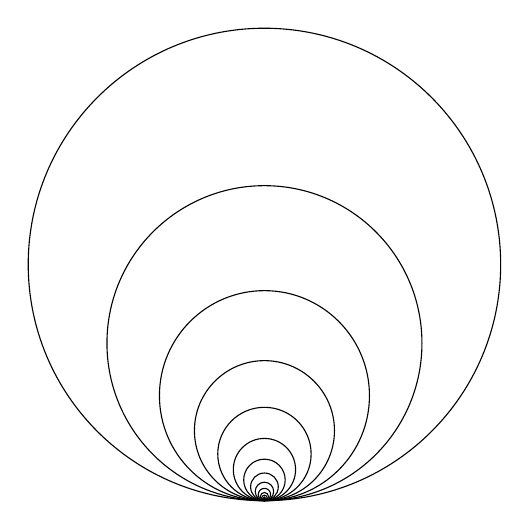
\begin{tikzpicture}
            \foreach \x in {0,...,30}{
                \pgfmathsetmacro\y{3*1.5^(-\x)}
                \draw (0, \y) circle [radius=\y cm];
            }
        \end{tikzpicture}
    \end{center}
    This space is not semi-locally simply connected. % why?
\end{eg}

Fortunately, all reasonable spaces are semi-locally simply connected, for instance cell complexes. For the rest of this course, all spaces are locally path-connected and semi-locally simply connected.

Construction of $\widetilde{X} \to X$ (universal cover)
Observation: Points in $\widetilde{X}$ <-> homotopy classes of paths in $X$ starting at $x_0$.

So set $\widetilde{X} = $
% stufff

% 3.3.1
\begin{thm}
    If $X$ is path connected and locally path connected, and semilocally simply connected then the universal cover
    \begin{equation*}
        p: \widetilde{X} \to X
    \end{equation*}
    exists.
\end{thm}

% remark path connected does not imply locally path connected eg join up topologists sine curve
\begin{proof}
    Omitted.
\end{proof}

% 3.4
\subsection{The Galois correspondence}
Given a based covering space $(\overline{X}, \overline{x}_0) \to (X, x_0)$, we get a subgroup $p_* \pi_1(\overline{X}, \overline{x}_0 \leq \pi_1(X, x_0)$.

Suppose $\overline{x}_0, \overline{x}_0' \in p^{-1} (x_0)$, we'd like to compare $p_* \pi_1 (\overline{X}, \overline{x}_0)$ and $p_* \pi_1 (\overline{X}, \overline{x}_0')$.
Can choose a path $\overline{\gamma} : \overline{x_0} \leadsto \overline{x}_0'$. Then, we see that $p_* \pi_1 (\overline{X}, \overline{x}_0)$ and $p_* \pi_1 (\overline{X}, \overline{x}_0')$ are conjugates via the element $[\gamma] \in \pi_1(X, x_0)$.

Given a unbased covering space, we get a conjugacy class of subgroup, represented by $p_* \pi_1(\overline{X},\overline{x}_0)$ for any $\overline{x}_0 \in p^{-1}(x_0)$.

The goal now is to improve these maps to bijections.
% see pic

To make sense of this, we need a notion of equivalence for covering spaces.

\begin{defi}
    An isomorphism of covering spaces is a pair of homeomorphisms
    \begin{equation*}
        \begin{tikzcd}
            \overline{X}_1 \arrow[r, "\phi"] & \overline{X}_2 \arrow[l, "\psi"']
        \end{tikzcd}
    \end{equation*}
    with $\phi = \psi^{-1}$ such that $p_2 \circ \phi = p_1$ and $p_1 \circ \psi = p_2$.
    \begin{equation*}
        \begin{tikzcd}
            \overline{X}_1 \arrow[rr, "\phi"] \arrow[rd, "p_1"] & & \overline{X}_2 \arrow[ll, "\psi"'] \arrow[ld, "p_2"] \\
                                             & X &
        \end{tikzcd}
    \end{equation*}
\end{defi}

\begin{defi}
    If $p: \overline{X} \to X$ is a covering space, a covering transofmation or deck transformation is a self-homoemorphism $\phi: \overline{X} \to \overline{X}$ such that $p \circ \phi = p$.
    In particular, $\phi$ is a lift of $p$ along itself, and so if $\overline{X}$ is path connected, $\phi$ is determined by its value at a point.

    \begin{equation*}
        \begin{tikzcd}
            \overline{X} \arrow[rr, "\phi"] \arrow[rd, "p"] & & \overline{X} \arrow[ld, "p"] \\
                                             & X &
        \end{tikzcd}
    \end{equation*}
\end{defi}

The following result is really useful.
% \begin{lemma}[Lifting Criterion]
%     Consider maps of based spaces
%     \begin{equation*}
%         \begin{tikzcd}
%             & (\overline{X}, \overline{x}_0) \ar[d, "p"] \\
%             (Y, y_0)
%         \end{tikzcd}
%     \end{equation*}
%     % finish
%
%     % lift exists iff
% \end{lemma}

% switch back to widetilde from overline

\begin{proof}
    $(\implies)$ If the lift $\widetilde{f}$ exists, $f_* = p_* \circ \widetilde{f}_* \implies \mathrm{im} f_* \subseteq \mathrm{im} p_*$

    $(\impliedby)$ Suppose $f_* \pi_1(Y, y_0) \subseteq p_* \pi_1 (\widetilde{X}, \widetilde{x}_0)$. For each $y \in Y$, choose $\alpha_y: y_0 \leadsto y$.
    Let $\widetilde{\alpha}_y$ be the unique lift of $f \circ \alpha_y$ to a path $I \to \widetilde{X}$ starting at $\widetilde{x}_0$.
    We would like to define $\widetilde{f}(y) = \widetilde{\alpha}_y(1)$, but this depends on our choice of $\alpha_y$.

    % diagram
    So, let $\beta_y : y_) \leadsto y$ be a different choice of path.

    Note that $\alpha_y \cdot \overline{\beta_y}$ is a loop in $Y$ based at $y_0$, and observe $f \circ (a_y \cdot \overline{\beta_y})$ is a loop in $X$, based at $x_0$. Therefore, by the hypothesis, $f \circ (\alpha_y \cdot \overline{\beta_y})$ is the image of some loop $\widetilde{\gamma}$ in $\widetilde{X}$. Hence $\widetilde{\alpha}_y$ and $\widetilde{\beta}_y$ form a loop in $\widetilde{X}$, and so have the same endpoints. So it makes sense to define $\widetilde{f}(y) = \widetilde{\alpha}_y$.
\end{proof}

The next tool is another action of $\pi_1(X, x_0)$.
Let $p : (\widetilde{X}, \widetilde{x}_0) \to (X, x_0)$ be a universal cover. For each $[\gamma] \in \pi_1(X, x_0)$, we can consider $\widetilde{x}_0 \cdot [\gamma]$ as a different choice of basepoint for $\widetilde{X}$.
The Lifting Criterion gives a (ubique) covering transofmation $\phi_{[\gamma]} : \widetilde{X} \to \widetilde{X}$.

\begin{lemma}
    This defines a left action of $\pi_1(X, x_0)$ on $\widetilde{X}$ by covering transformation.
\end{lemma}

\begin{proof}
    We need to check that for $[\alpha], [\beta] \in \pi_1(X, x_0)$,
    \begin{equation*}
        \phi_\alpha \circ \phi_\beta = \phi_{\alpha \cdot \beta}
    \end{equation*}
    Note $\phi_\alpha^{-1} \circ \widetilde{\beta}_{\widetilde{x}_0 \cdot [\alpha]}$ is a lift of $\beta$ at $\widetilde{x}_0$, hence = $\widetilde{\beta}_{\widetilde{x}_0}$.
    Hence $\phi_\alpha^{-1} \circ \widetilde{\beta}_{\widetilde{x}_0 \cdot [\alpha]}(1) =\widetilde{\beta}_{\widetilde{x}_0}(1) = \phi_\beta (\widetilde{x}_0)$
    \begin{align*}
        \phi_\alpha \circ \phi_\beta (\widetilde{x}_0) &= \widetilde{\beta}_{\widetilde{x}_0 \cdot [\alpha]}(1) \\
                                                       &= \widetilde{\alpha \cdot \beta}_{\widetilde{x}_0} (1) \\
                                                       &= \phi_{\alpha \cdot \beta}(\widetilde{x}_0)
    \end{align*}
    So $\phi_\alpha \circ \phi_\beta$ by uniqueness.
\end{proof}

Surjectivity of Galois correspondence.

Given $H \geq \pi_1(X, x_0)$, we want to construct a covering map
\begin{equation*}
    p_H:(X^H, x_0^H) \to (X, x_0)
\end{equation*}
such that $(p_H)_* \pi_1(X^H, x_0^H) = H$. For instance, if $H = 1$ then

% missing stuff

\clearpage
% section4
\section{Some Group Theory}
Our goal is to compute more fundamental groups, for instance with a `gluing theorem' relating $\pi_1 X$ to $\pi_1 A$, $\pi_1 B$, $\pi_1 C$ with $X = A \cup_C B$.
\begin{center}
    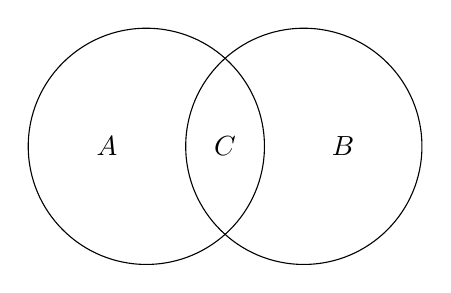
\begin{tikzpicture}[scale=0.5]
        \draw (0, 0) circle [radius=3cm];
        \draw (4, 0) circle [radius=3cm];
        \node at (-1, 0) {$A$};
        \node at (2, 0) {$C$};
        \node at (5, 0) {$B$};
    \end{tikzpicture}
\end{center}
Our intuition says that $\pi_1 X$ is glued together out of  $\pi_1 A$, $\pi_1 B$, $\pi_1 C$, but we have no idea what gluing of groups means.

\subsection{Free groups and presentations}
Let $S$ be a set, called the alphabet (for instance $S = \{a, b\}$).
Let $S^{-1} = \set{s^{-1} | s \in S}$, the formal inverses, so $S^{-1} \cap S = \emptyset$.

Let $S^* = \set{\text{words in } S \cup S^{-1}} = \set{s_1^\pm s_2^\pm \dotsm s_n^\pm | s_i \in S, n \geq 0}$, noting that the empty word is a word.
Continuing the example, $w = a b b^{-1} a b^{-1} a^{-1} a$ is a word.

An elementary reduction on a word $w = u \cdot s^\pm \cdot s^\mp \cdot v \leadsto u \cdot v$.
If no elementary reductions are possible, $w$ is called reduced.

\begin{defi}
    The \textbf{free group on $S$}, $F(S)$ is the set of reduced words in $S^*$ equipped with the following group operation:
    \begin{equation*}
        w_1 , w_2 \leadsto w_1 \cdot w_2 \leadsto u
    \end{equation*}
    where we first concatenate, then perform elementary reductions.
    We will see later that this is well defined.
\end{defi}

For instance, take $w_1 = a^2 b^{-1}$ and $w_2 = b a^{-1} b^{-1}$, so $w_1 w_2 = a^2 b^{-1} b a^{-1} b^{-1} = a^2 a^{-1} b^{-1} = a b^{-1}$.
Note there is a canonical set map $S \to F(S)$.

% lem 4.1.2
\begin{lemma}[Universal property of free groups]
    For any set map $\phi:S \to H$, with $H$ a group, there is a unique homomorphism $f: F(S) \to H$ such that
    \begin{equation*}
        \begin{tikzcd}
            F(S) \arrow[rd, dashed, "\exists! f"] & \\
            S \arrow[u] \arrow[r, "\phi"] & H
        \end{tikzcd}
    \end{equation*}
    commutes.
\end{lemma}

\begin{proof}
    For $w = s_1^\pm \dotsm s_n^\pm$, let $f(w) = \phi(s_1)^\pm \dotsm \phi(s_n)^\pm$. Note that if $w \leadsto v$ via an elementary reduction then $f(w) = f(v)$.
\end{proof}

\begin{remark}
    By this lemma, $F(S)$ is unique up to canonical isomorphism.
\end{remark}

\begin{notation}
    If $G$ is a group and $R \subseteq G$ then $\langle\langle R \rangle\rangle$ is the smallest normal subgroup containing $R$.
\end{notation}

% 4.1.3
\begin{defi}
    Let $R \subseteq F(S)$. The data $(S, R)$ is called a \textbf{presentation}, and elements of $R$ are called relations.
    If $S, R$ are both finite, we say that $(S, R)$ is finite. Now,
    \begin{equation*}
        \langle S | R \rangle \coloneqq F(S) / \langle\langle R \rangle \rangle
    \end{equation*}

    If $(S, R)$ is finite, we say $\langle S|R\rangle$ is \textbf{finitely presented}.
\end{defi}

% 4.1.4
\begin{lemma}[Universal property of presentations]
    For any set map $\phi:S \to H$, with $H$ a group such that $\forall r \in R, \phi(r) = 1$, there is a unique homomorphism $f: \langle S | R \rangle \to H$ such that
    \begin{equation*}
        \begin{tikzcd}
            \langle S | R \rangle \arrow[rd, dashed, "\exists! f"] & \\
            S \arrow[u] \arrow[r, "\phi"] & H
        \end{tikzcd}
    \end{equation*}
    commutes.
\end{lemma}
\begin{proof}
    Easy exercise.
\end{proof}

% 4.1.5
\begin{eg}[The stupid presentation]
    Let $G$ be a group. Let $S = G$, let $\phi: G \to G$ be the identity.
    Then $\exists!$ canonical $F(G) \xrightarrow{\eta} G$.
    Let $R = \mathrm{ker} \eta$. In particular, $\langle\langle R \rangle \rangle = R$, and the isomorphism theorem gives $G \cong \langle G | R \rangle$.
\end{eg}

% 4.1.7
\begin{eg}
    $G = \langle a, b | a b^{-3}, b a^{-2} \rangle$.
    We have $a = b^3$ so $a = (a^2)^3 = a^6$ hence $a^5 = 1$ and $b = a^2$, so every element of $G$ is a product of $a$'s.
    So the elements of the group are represented in $1, a, a^2, a^3, a^4$.
    $\abs{G} \leq 5$, and we guess $G \cong \Z/5\Z$. To prove this, let
    \begin{align*}
        \phi:\{a, b\} &\rightarrow \Z/5\Z \\
        a &\longmapsto 1 \\
        b &\longmapsto 2 \\
    \end{align*}
    so $\phi(b^3) = \phi(b)^3 = 3 \times 2 = 6 = 1 = \phi(a)$ and $\phi(a)^2 = 2 \times 1 = 2 = \phi(b)$.
    By the universal property of presentations, there is a homomorphism $f: G \to \Z/5\Z$, containing $1 \in \mathrm{im} f \implies f$ surjective. Thus $\abs{G} = 5$ and $f$ is an isomorphism.
\end{eg}

\subsection{Another view of free groups}

% 5.1.14 wtf
\begin{eg}
    Let $X$ be the wedge of two circles
\end{eg}

% stuff missing

% 6.2.6
\begin{lemma}
    $K$ a simplicial complex, $n$ max dimension of a simplex of $K$.
    \begin{equation*}
        \mu(K^{(r)}) \leq \frac{n}{n+1}^r \mu(K).
    \end{equation*}
\end{lemma}

\begin{proof}
    The general result follows from the case $r=1$ by induction.
    Let $\tau \leq \sigma \in K$. We need to bound $\norm{\hat{\tau} - \hat{\sigma}}$ from above. Note that if $\sigma = \langle a_0, \dotsc, a_m \rangle$ then
    \begin{align*}
        \norm{\hat{\tau} - \hat{\sigma}} &\leq \max_{i=0, \dotsc, m} \norm{a_i - \hat{\sigma}} \\
                                         &= \norm{a_0 - \hat{\sigma}} \text{wlog} \\
                                         &= \norm{a_0 - \frac{1}{m+i} \sum_{i=0}^m a_i} \\
                                         &= \frac{1}{m+1} \norm{\sum_{i=1}^m a_0 - a_i} \\
                                         &\leq \frac{1}{m+1} \sum_{i=1}^m \norm{a_0 - a_i}  \\
                                         &\leq \frac{m}{m+1} \mu(K) \\
                                         &\leq \frac{n}{n+1} \mu(K) \qedhere
    \end{align*}
\end{proof}

We'll use this to prove
% 6.2.7
\begin{thm}[Simplicial Approximation Theorem]
    If $f: \abs{K} \to \abs{L}$ is a continuous map between polyhedra, there is an $r \leq 0$ and a simplicial approximation $g: V_{k^{(r)}} \to V_L$ to $f$ (and relative statement).
\end{thm}

\begin{proof}
    Consider $\set{St_L(w) | w \in V_L}$ a (finite) open cover of $\abs{L}$.
    Therefore $\set{f^{-1} St_L(w) | w \in V_L}$ is a finite open cover $\abs{K}$.
    Now use the lebesgue number lemma, which states
    \begin{equation*}
        \exists \delta > 0 such that \forall x \in \abs{K} B_x(\delta) \subseteq f^{-1} St_L(w) for some w \in V_L
    \end{equation*}
    By lemma 6.2.6 for $r$ sufficiently large, $\mu(K^{(r)}) < \delta$.
    Now for every $v \in V_{k^{(r)}}$, $St_{K^{(r)}(v)} \subseteq B_v(\delta) \subseteq f^{-1} St_L(w) \implies$ the result, setting $g(v)$ to be any such $w$.
    For the relative statement, if $f|_N$ is simplicial, choose $w = f(v)$ for $v \in V_N$ and make $\delta$ slightly smaller.
\end{proof}

% section 7
\section{Homology}
\subsection{Simplicial homology}
Consider $K$-simplicial complex.

\begin{defi}
    An oriented simplex $\sigma$ is an (n+1)-tuple of vertices $(a_0, \dotsc, a_n)$ up to equivalence:
    \begin{enumerate}[label=(\roman*)]
        \item $\langle a_0, \dotsc, a_n \rangle \in K$
        \item for any even permutation $\pi$ of $\{0, \dotsc, n\}$, $(a_0, \dotsc, a_n) \sim (a_{\pi(0)}, \dotsc, a_{\pi(n)})$.
            For any odd permutation $\pi$ of $\{0, \dotsc, n\}$, we write
            $\overline{\sigma} = (a_{\pi(0), \dotsc, a_{\pi(n)}})$, the same simplex with the opposite orientation.
    \end{enumerate}
\end{defi}

\begin{eg}
    For $n=1$, $\sigma = \langle a_0, a_1 \rangle$
    % finish w/ picture
\end{eg}

\begin{defi}
    For each simplex $\sigma$ of $K$, fix an orientation on $\sigma$.
    Define $C_n(K) = \bigoplus \Z \sigma$ for $n \geq 0$, where the sum is over $\sigma$ an $n$-simplex of $K$.
    So we write things like $3 \sigma_1 - 2 \sigma_2$.
    We identify $-\sigma = \overline{\sigma}$ for each $\sigma$.
    This is called the nth chain group of $K$. For $n < 0$, set $C_n(K) = 0$.
\end{defi}

\begin{defi}
    We define the boundary homomorphism
    $d_n: C_n(K) \to C_{n-1}(K)$
    defined by $(a_0, \dotsc, a_n) \mapsto \sum_{i=0}^n (-1)^i (a_0, \dotsc, \hat{a_i}, \dotsc, a_n)$, where
    $(a_0, \dotsc, \hat{a_i}, \dotsc, a_n)$ means $(a_0, \dotsc, a_{i-1}, a_{i+1}, \dotsc, a_n)$.
\end{defi}

\begin{eg}
    $(a_0, a_1) \mapsto (-1)^0 (\hat{a_0}, a_1) + (-1)^1 (a_0, \hat{a_1}) = (a_1 - a_0)$
    % picture

    $\sigma = (a_0, a_1, a_2) \mapsto (a_1, a_2) - (a_0, a_2) + (a_0, a_1) = (a_1, a_2) + (a_2, a_0) + (a_0, a_1)$.

    % more picture
\end{eg}

\begin{lemma}
    \begin{equation*}
        d_{n-1} \circ d_n = 0
    \end{equation*}
\end{lemma}

\begin{proof}
    It's enough to check that $d_{n-1} \circ d_n(\sigma) = 0$ for $\sigma = (a_0, \dotsc, a_n)$.
    We see that $d_{n-1} \circ d_n(\sigma)= \sum_{j < i} (-1)^{i+j} (a_0, \dotsc, \hat{a_j}, \dotsc, \hat{a_i}, \dotsc, a_n) + \sum_{j > i} (-1)^{i+j} (a_0, \dotsc, \hat{a_i}, \dotsc, \hat{a_j}, \dotsc, a_n) = 0$.
\end{proof}
\end{document}
